\chapter{El agua y las biomoléculas pequeñas}\label{ch:b1:water-small-molecules}

Una bacteria de un micrómetro cúbico contiene unos veinte mil millones de
moléculas de agua y unos pocos cientos de millones de todo lo demás. El agua
no es el telón de fondo de la \omterm{def:b1:cell-unit-of-life:cell}{célula}, sino su medio: disuelve los iones y
los azúcares, esconde las partes aceitosas de las proteínas y de las
membranas, fija la acidez de la que depende toda enzima, y es reactivo o
producto en la mitad de las reacciones del metabolismo. Este capítulo
describe el agua y los enlaces débiles que forma y rompe, la aritmética de
los ácidos, las \omterm{def:b1:water-small-molecules:ph}{bases} y los tampones, las moléculas orgánicas pequeñas con
las que se construyen las macromoléculas de los cuatro capítulos siguientes,
y la moneda de la energía --- el \omterm{def:b1:water-small-molecules:atp}{ATP} --- con la que la \omterm{def:b1:cell-unit-of-life:cell}{célula} paga su
construcción.

\section{El agua}

\begin{definition}[La molécula de agua]\label{def:b1:water-small-molecules:water}
\index{agua}
El agua, $\mathrm{H_2O}$, es una molécula angular (el ángulo H--O--H es de
$104.5^\circ$) en la que el oxígeno atrae hacia sí los electrones
compartidos: es \emph{polar}\index{molécula polar}, con una carga parcial
negativa sobre el oxígeno y cargas parciales positivas sobre los hidrógenos.
Cada molécula puede formar hasta cuatro \emph{enlaces de
hidrógeno}\index{enlace de hidrógeno} --- una atracción electrostática entre
un hidrógeno unido a un átomo electronegativo (O, N) y un par no compartido
de otro átomo electronegativo ---, dos por sus hidrógenos y dos por su
oxígeno. El agua líquida es una red de esos enlaces, cada uno de los cuales
dura unos picosegundos.
\end{definition}

\begin{omfigure}
\begin{tikzpicture}[font=\small, line cap=round,
  O/.style={circle, draw, thick, fill=omThm!30, minimum size=8mm, inner sep=0pt},
  H/.style={circle, draw, thick, fill=gray!15, minimum size=5.5mm, inner sep=0pt}]
  % central water molecule
  \node[O] (O) at (0,0) {O};
  \node[H] (H1) at (-0.8,-0.7) {H};
  \node[H] (H2) at (0.8,-0.7) {H};
  \draw[thick] (O) -- (H1); \draw[thick] (O) -- (H2);
  \node[font=\scriptsize, omThm] at (0,0.62) {$\delta^-$};
  \node[font=\scriptsize] at (-1.4,-0.55) {$\delta^+$};
  \node[font=\scriptsize] at (1.4,-0.55) {$\delta^+$};
  % lower-left neighbour (accepts an H bond from H1)
  \node[O] (O2) at (-2.1,-2.3) {O};
  \node[H] (H2a) at (-3.05,-2.55) {H};
  \node[H] (H2b) at (-1.75,-3.3) {H};
  \draw[thick] (O2) -- (H2a); \draw[thick] (O2) -- (H2b);
  \draw[dashed, thick, omDef] (H1) -- (O2);
  % lower-right neighbour
  \node[O] (O3) at (2.1,-2.3) {O};
  \node[H] (H3a) at (3.05,-2.55) {H};
  \node[H] (H3b) at (1.75,-3.3) {H};
  \draw[thick] (O3) -- (H3a); \draw[thick] (O3) -- (H3b);
  \draw[dashed, thick, omDef] (H2) -- (O3);
  % upper-left neighbour (donates an H bond to O)
  \node[H] (H4) at (-1.1,1.55) {H};
  \node[O] (O4) at (-2.0,2.25) {O};
  \node[H] (H4b) at (-2.95,2.6) {H};
  \draw[thick] (O4) -- (H4); \draw[thick] (O4) -- (H4b);
  \draw[dashed, thick, omDef] (H4) -- (O);
  % upper-right neighbour
  \node[H] (H5) at (1.1,1.55) {H};
  \node[O] (O5) at (2.0,2.25) {O};
  \node[H] (H5b) at (2.95,2.6) {H};
  \draw[thick] (O5) -- (H5); \draw[thick] (O5) -- (H5b);
  \draw[dashed, thick, omDef] (H5) -- (O);
  \node[anchor=west, align=left, font=\footnotesize] at (4.0,1.0) {discontinuo: enlaces de hidrógeno\\ (\qty{0.18}{nm}, unos \qty{20}{kJ/mol} cada uno)\\ continuo: enlaces covalentes O--H\\ (\qty{0.096}{nm}, \qty{460}{kJ/mol})};
  \node[anchor=west, align=left, font=\footnotesize] at (4.0,-1.3) {cada molécula cede dos enlaces\\ de hidrógeno y acepta otros dos:\\ una red tetraédrica};
\end{tikzpicture}

{\small Una molécula de agua (ángulo H--O--H de $104.5^\circ$) y sus cuatro
vecinas unidas por \omterm{def:b1:water-small-molecules:water}{enlaces de hidrógeno}. La molécula angular y \omterm{def:b1:water-small-molecules:water}{polar} cede dos \omterm{def:b1:water-small-molecules:water}{enlaces de hidrógeno} por sus hidrógenos
y acepta dos sobre su oxígeno; la red que forman da al agua su cohesión, su
capacidad calorífica y su poder como disolvente.}
\end{omfigure}

\begin{proposition}[Propiedades del agua que importan a la vida]\label{prop:b1:water-small-molecules:properties}
La red de \omterm{def:b1:water-small-molecules:water}{enlaces de hidrógeno} explica las propiedades excepcionales del agua:
\begin{itemize}
  \item una elevada \emph{cohesión} y tensión superficial (\qty{72}{mN/m}):
        las columnas de agua pueden ascender por un árbol sin romperse
        (\cref{ch:b1:plant-transport}); los insectos caminan sobre las
        charcas;
  \item una elevada \emph{capacidad calorífica}
        (\qty{4.18}{kJ.kg^{-1}.K^{-1}}) y un elevado calor de vaporización
        (\qty{2.4}{kJ/g}): las temperaturas de los \omterm{def:b1:organism-environment:organism}{organismos} y de las
        masas de agua cambian despacio, y evaporar un gramo de sudor
        retira \qty{2.4}{kJ};
  \item un \emph{sólido menos denso que el líquido}: el hielo flota, y los
        lagos se congelan de arriba abajo y dejan agua líquida debajo;
  \item un excelente \emph{disolvente} de iones y \omterm{def:b1:water-small-molecules:water}{moléculas polares}, a los
        que rodea con capas orientadas (\emph{hidratación}), y muy malo
        para las moléculas apolares, a las que fuerza a juntarse (el
        \emph{efecto hidrófobo}\index{efecto hidrófobo}).
\end{itemize}
\end{proposition}
\begin{proof}[Demostración parcial]
La cohesión y la tensión superficial miden el trabajo de separar moléculas
retenidas cada una por cuatro enlaces de unos \qty{20}{kJ/mol}. Calentar el
agua exige romper enlaces además de agitar moléculas: de ahí la capacidad
calorífica; vaporizarla exige romperlos todos. El hielo mantiene cada
molécula en una red tetraédrica abierta de cuatro enlaces, que ocupa más
volumen que el líquido desordenado, en el que las moléculas se empaquetan
más juntas. Los iones y los grupos \omterm{def:b1:water-small-molecules:water}{polares} se estabilizan por \omterm{def:b1:water-small-molecules:water}{enlaces de
hidrógeno} con el agua; una molécula apolar no puede formarlos, y el agua que
la rodea debe ordenarse en una jaula, con un coste de entropía que
disminuye cuando las moléculas apolares se agrupan y comparten una jaula.
\end{proof}

\begin{omfigure}
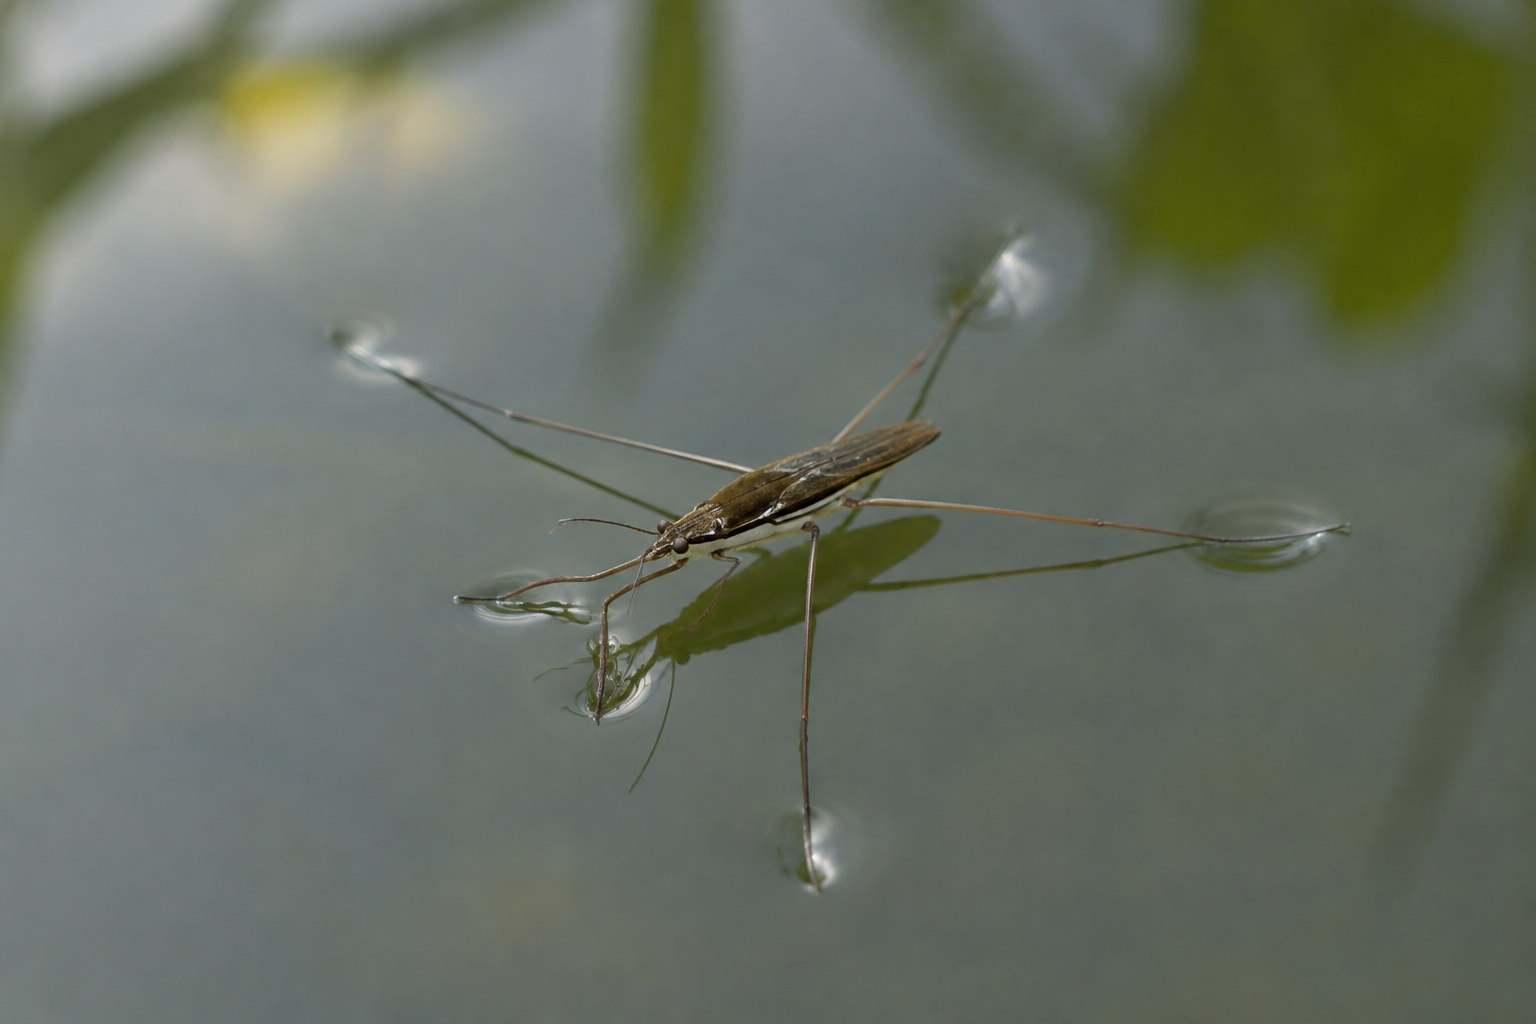
\includegraphics[width=0.6\linewidth]{images/book3/ai/b3-08-water-strider.png}

{\small Un zapatero sobre una charca: los hoyuelos bajo sus patas son la
superficie mantenida tensa por la cohesión del agua unida por \omterm{def:b1:water-small-molecules:water}{enlaces de
hidrógeno}.}
\end{omfigure}

\begin{example}[El efecto hidrófobo en acción]\label{ex:b1:water-small-molecules:hydrophobic}
Agítese aceite en agua y en unos minutos las gotitas se habrán fundido: el
agua expulsa aquello con lo que no puede enlazarse. El mismo efecto pliega
una proteína (sus residuos aceitosos se esconden dentro,
\cref{ch:b1:proteins}), ensambla una membrana (las colas de los lípidos se
reúnen lejos del agua, \cref{ch:b1:lipids}) y junta dos superficies
moleculares complementarias. Nada atrae el aceite hacia el aceite: es el
agua la que empuja.
\end{example}

\section{Enlaces débiles}

\begin{definition}[Enlaces covalentes y no covalentes]\label{def:b1:water-small-molecules:bonds}
Un \emph{enlace covalente}\index{enlace covalente} comparte un par de
electrones entre dos átomos y cuesta \qtyrange{300}{500}{kJ/mol} romperlo:
los esqueletos de las moléculas son covalentes, y en la \omterm{def:b1:cell-unit-of-life:cell}{célula} solo las
enzimas los forman o los rompen. Los \emph{enlaces no
covalentes}\index{enlace no covalente} son las atracciones débiles y
reversibles que mantienen unas moléculas \emph{unidas a otras} y les dan
forma: el \emph{\omterm{def:b1:water-small-molecules:water}{enlace de hidrógeno}} (\qtyrange{4}{20}{kJ/mol} en agua); el
\emph{enlace iónico}\index{enlace iónico} entre cargas opuestas (unos
\qty{12}{kJ/mol} en agua, cuya constante dieléctrica apantalla las cargas
ochenta veces); las atracciones de \emph{van der Waals}\index{fuerza de van der Waals} entre dos átomos cualesquiera en contacto estrecho
(\qtyrange{1}{4}{kJ/mol} cada una, pero sumadas sobre toda una superficie);
y el \emph{\omterm{prop:b1:water-small-molecules:properties}{efecto hidrófobo}}, que no es un enlace, sino la exclusión de las
superficies apolares por parte del agua.
\end{definition}

\begin{proposition}[Por qué los enlaces débiles son los enlaces de la biología]\label{prop:b1:water-small-molecules:weak}
La energía térmica a \qty{37}{\celsius} es $RT = \qty{2.6}{kJ/mol}$. Un
único enlace débil es solo unas pocas veces mayor y se rompe en
microsegundos; diez juntos, sobre dos superficies que encajan, aguantan
horas. El \emph{reconocimiento}\index{reconocimiento molecular} molecular
--- de una enzima por su sustrato, de un anticuerpo por su antígeno, de una
hebra de ADN por su complementaria --- descansa sobre muchos enlaces débiles
formados a la vez entre superficies complementarias, y por eso es a un
tiempo específico (solo una superficie que encaje los forma todos) y
reversible (el calor, o un competidor, lo deshace). Los \omterm{def:b1:water-small-molecules:bonds}{enlaces covalentes},
cien veces más fuertes, serían permanentes.
\end{proposition}

\begin{example}[Fundir una doble hélice]\label{ex:b1:water-small-molecules:melting}
Las dos hebras del ADN se mantienen unidas por dos o tres \omterm{def:b1:water-small-molecules:water}{enlaces de
hidrógeno} por par de \omterm{def:b1:water-small-molecules:ph}{bases} más el apilamiento (\omterm{def:b1:water-small-molecules:bonds}{van der Waals}) de los pares
vecinos; un par aislado se separaría al instante, pero mil pares seguidos
aguantan hasta que la temperatura alcanza unos \qty{90}{\celsius}, y se
reúnen, exactamente en el mismo registro, cuando se baja
(\cref{ch:b1:nucleic-acids}). Específico, fuerte por acumulación,
reversible.
\end{example}

\section{Ácidos, bases y tampones}

\begin{definition}[pH, ácido, base, p$K_a$]\label{def:b1:water-small-molecules:ph}
El agua se disocia ligeramente, $\mathrm{H_2O} \rightleftharpoons
\mathrm{H^+} + \mathrm{OH^-}$, con $[\mathrm{H^+}][\mathrm{OH^-}] =
K_w = \qty{e-14}{mol^2/L^2}$ a \qty{25}{\celsius}. El \emph{pH}\index{pH}
es $-\log_{10}[\mathrm{H^+}]$: 7 para el agua pura, menor para los ácidos y
mayor para las bases. Un \emph{ácido}\index{ácido} $\mathrm{HA}$ cede un
protón, $\mathrm{HA} \rightleftharpoons \mathrm{H^+} +
\mathrm{A^-}$, con
constante de disociación $K_a =
[\mathrm{H^+}][\mathrm{A^-}]/[\mathrm{HA}]$ y
\emph{p$K_a$}\index{pKa@p$K_a$} $= -\log_{10}K_a$; su \emph{base}\index{base}
conjugada $\mathrm{A^-}$ acepta uno. Un ácido fuerte (HCl) está totalmente
disociado; los ácidos de la \omterm{def:b1:cell-unit-of-life:cell}{célula} (ácidos carboxílicos, fosfatos, amonio)
son débiles, con p$K_a$ entre 2 y 10.
\end{definition}

\begin{theorem}[Henderson--Hasselbalch]\label{thm:b1:water-small-molecules:hh}
\index{ecuación de Henderson--Hasselbalch}
Para un ácido débil en disolución,
\[
\mathrm{pH} = \mathrm{p}K_a + \log_{10}\frac{[\mathrm{A^-}]}{[\mathrm{HA}]} .
\]
Cuando $\mathrm{pH} = \mathrm{p}K_a$ el ácido está disociado a la mitad; una
unidad de \omterm{def:b1:water-small-molecules:ph}{pH} por encima está disociado al \qty{91}{\%}, y una por debajo, al
\qty{9}{\%}.
\end{theorem}
\begin{proof}
Tómese el logaritmo de $K_a = [\mathrm{H^+}][\mathrm{A^-}]/[\mathrm{HA}]$:
$\log K_a = \log[\mathrm{H^+}] + \log([\mathrm{A^-}]/[\mathrm{HA}])$, es
decir, $-\mathrm{p}K_a = -\mathrm{pH} + \log([\mathrm{A^-}]/[\mathrm{HA}])$.
El cociente vale $1$, $10$ y $0.1$ a \omterm{def:b1:water-small-molecules:ph}{pH} $= \mathrm{p}K_a$, $\mathrm{p}K_a + 1$
y $\mathrm{p}K_a - 1$.
\end{proof}

\begin{definition}[Tampón]\label{def:b1:water-small-molecules:buffer}
Un \emph{tampón}\index{tampón} es una disolución que contiene un ácido débil
y su \omterm{def:b1:water-small-molecules:ph}{base} conjugada en cantidades comparables; resiste los cambios de \omterm{def:b1:water-small-molecules:ph}{pH},
porque el $\mathrm{H^+}$ añadido lo capta $\mathrm{A^-}$ y el
$\mathrm{OH^-}$ añadido lo capta $\mathrm{HA}$. Funciona mejor dentro de una
unidad en torno a la p$K_a$, y su \emph{capacidad} crece con la
concentración total del par. Los tampones de la \omterm{def:b1:cell-unit-of-life:cell}{célula}: el fosfato
($\mathrm{H_2PO_4^-}/\mathrm{HPO_4^{2-}}$, p$K_a$ 6,8) y las cadenas
laterales de las proteínas dentro de las \omterm{def:b1:cell-unit-of-life:cell}{células}; el bicarbonato
($\mathrm{CO_2}/\mathrm{HCO_3^-}$, p$K_a$ efectiva 6,1) en la sangre, cuyo
socio ácido es un gas que los pulmones pueden retirar.
\end{definition}

\begin{omfigure}
\begin{tikzpicture}
\begin{axis}[
  width=0.86\linewidth, height=6.2cm,
  axis x line=bottom, axis y line=left,
  xmin=0, xmax=1, ymin=3, ymax=11,
  xlabel={fracción de ácido neutralizada (equivalentes de $\mathrm{OH^-}$ añadidos)}, ylabel={pH},
  xlabel style={font=\small, at={(axis description cs:0.5,-0.12)}, anchor=north},
  ylabel style={font=\small},
  tick label style={font=\small}, xtick={0,0.25,0.5,0.75,1}, ytick={3,4,5,6,7,8,9,10,11},
  clip=false,
]
\addplot[very thick, omDef, domain=0.02:0.98, samples=120] {6.8 + log10(x/(1-x))};
\draw[dashed, gray] (axis cs:0,6.8) -- (axis cs:0.5,6.8);
\draw[dashed, gray] (axis cs:0.5,3) -- (axis cs:0.5,6.8);
\node[font=\scriptsize, anchor=south west] at (axis cs:0.02,6.85) {pH $=$ p$K_a$ $= 6.8$ a la semineutralización};
\draw[<->, thick, omThm] (axis cs:0.09,5.8) -- (axis cs:0.91,7.8);
\node[font=\scriptsize, omThm, anchor=north west, align=left] at (axis cs:0.55,5.7) {intervalo tamponante:\\ p$K_a \pm 1$, curva plana};
\end{axis}
\end{tikzpicture}

{\small Valoración de un ácido débil (fosfato, p$K_a$ 6,8) por una \omterm{def:b1:water-small-molecules:ph}{base}. La
curva es plana en torno a la p$K_a$: allí, añadir \omterm{def:b1:water-small-molecules:ph}{base} cambia el cociente
entre \omterm{def:b1:water-small-molecules:ph}{base} y ácido, pero apenas el \omterm{def:b1:water-small-molecules:ph}{pH}. Fuera de ese intervalo el \omterm{def:b1:water-small-molecules:ph}{pH} oscila
libremente.}
\end{omfigure}

\begin{omfigure}
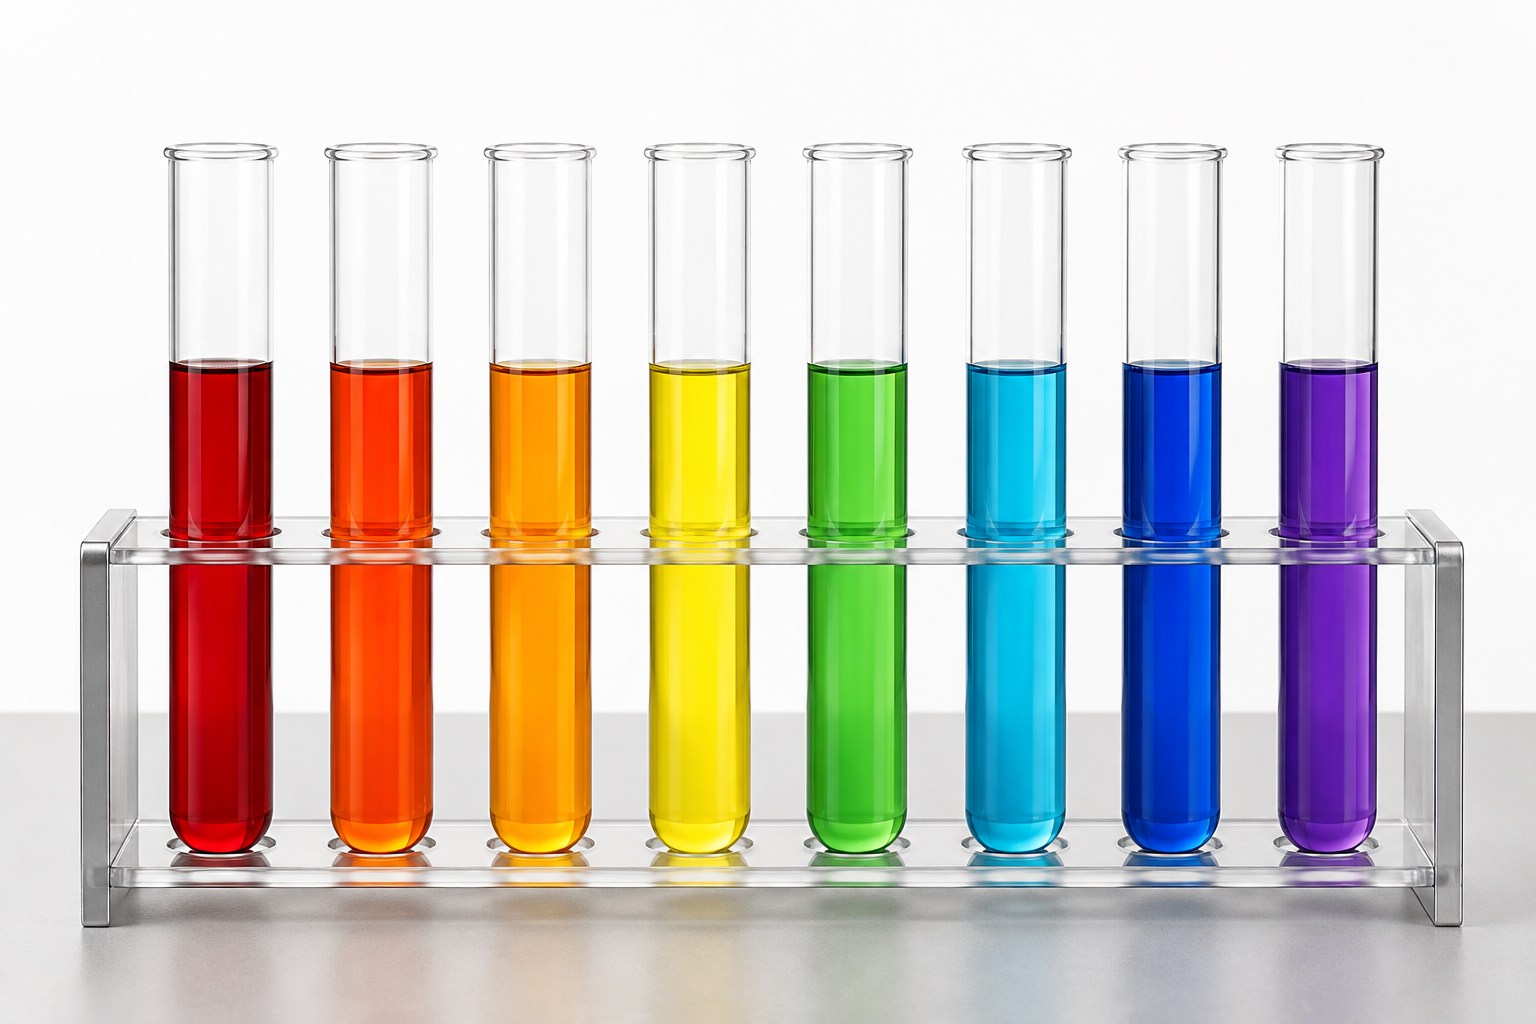
\includegraphics[width=0.6\linewidth]{images/book3/ai/b3-08-indicator-tubes.png}

{\small La escala de \omterm{def:b1:water-small-molecules:ph}{pH} hecha visible con un indicador universal: del rojo a
\omterm{def:b1:water-small-molecules:ph}{pH} 2 al violeta a \omterm{def:b1:water-small-molecules:ph}{pH} 12. El jugo gástrico está a 1--2, la orina a 5--8, la
sangre a 7,4, el intestino delgado a 8, el \omterm{def:b1:eukaryotic-cell:organelle}{citosol} a 7,2, el \omterm{def:b1:eukaryotic-cell:endomembrane}{lisosoma} a 5,
la luz del tilacoide con luz a 5 y el estroma a 8.}
\end{omfigure}

\begin{method}[Aritmética de los tampones]\label{met:b1:water-small-molecules:bufferarith}
\begin{enumerate}
  \item Identifíquense el par ácido--base y su p$K_a$ a la temperatura de
        trabajo.
  \item Aplíquese Henderson--Hasselbalch para obtener el cociente
        \omterm{def:b1:water-small-molecules:ph}{base}/ácido a partir del \omterm{def:b1:water-small-molecules:ph}{pH}, o el \omterm{def:b1:water-small-molecules:ph}{pH} a partir de las
        concentraciones.
  \item Para añadir un ácido fuerte: réstese su cantidad de la \omterm{def:b1:water-small-molecules:ph}{base} y
        súmese al ácido, y recalcúlese después el \omterm{def:b1:water-small-molecules:ph}{pH}. Para añadir una \omterm{def:b1:water-small-molecules:ph}{base}
        fuerte, al revés.
  \item Si uno de los socios puede salir del sistema (dióxido de carbono
        exhalado, amoniaco excretado), el sistema es \emph{abierto}:
        manténgase ese socio en su valor impuesto en vez de dejar que se
        acumule. Los tampones abiertos sostienen el \omterm{def:b1:water-small-molecules:ph}{pH} mucho mejor que los
        cerrados.
\end{enumerate}
\end{method}

\begin{example}[La sangre]\label{ex:b1:water-small-molecules:blood}
La sangre arterial contiene \qty{24}{mmol/L} de bicarbonato y
$\mathrm{CO_2}$ disuelto a \qty{1.2}{mmol/L} (fijado por los pulmones):
$\mathrm{pH} =
6.1 + \log(24/1.2) = 6.1 + 1.30 = 7.4$. Añadir
\qty{5}{mmol/L} de ácido convierte \qty{5}{mmol/L} de bicarbonato en
$\mathrm{CO_2}$; si los pulmones expulsan ese $\mathrm{CO_2}$ y mantienen el
valor disuelto, el \omterm{def:b1:water-small-molecules:ph}{pH} pasa a $6.1 + \log(19/1.2) = 7.30$; en un matraz
cerrado el $\mathrm{CO_2}$ subiría a \qty{6.2}{mmol/L} y el \omterm{def:b1:water-small-molecules:ph}{pH} caería a
$6.1 + \log(19/6.2) =
6.59$. Los pulmones marcan la diferencia.
\end{example}

\section{Biomoléculas pequeñas}

\begin{definition}[Grupos funcionales]\label{def:b1:water-small-molecules:groups}
Las moléculas orgánicas de la \omterm{def:b1:cell-unit-of-life:cell}{célula} son esqueletos de carbono que llevan un
pequeño repertorio de \emph{grupos funcionales}\index{grupo funcional} que
determinan su química:
\begin{center}
\small
\begin{tabular}{llll}
\hline
grupo & fórmula & propiedad & se encuentra en \\
\hline
hidroxilo & $-\mathrm{OH}$ & \omterm{def:b1:water-small-molecules:water}{polar}, forma enlaces de H & azúcares, alcoholes \\
carbonilo & $>\!\mathrm{C{=}O}$ & \omterm{def:b1:water-small-molecules:water}{polar}, reactivo & aldosas, cetosas \\
carboxilo & $-\mathrm{COOH}$ & ácido (p$K_a \approx 4$) & ácidos grasos, aminoácidos \\
amino & $-\mathrm{NH_2}$ & \omterm{def:b1:water-small-molecules:ph}{base} (p$K_a \approx 9$) & aminoácidos \\
fosfato & $-\mathrm{OPO_3^{2-}}$ & con carga, enlaces ricos en energía & nucleótidos, \omterm{def:b1:water-small-molecules:atp}{ATP} \\
sulfhidrilo & $-\mathrm{SH}$ & forma puentes S--S & cisteína \\
metilo & $-\mathrm{CH_3}$ & apolar & lípidos, marcas del ADN \\
\hline
\end{tabular}
\end{center}
Al \omterm{def:b1:water-small-molecules:ph}{pH} de la \omterm{def:b1:cell-unit-of-life:cell}{célula} los grupos carboxilo están ionizados
($-\mathrm{COO^-}$) y los grupos amino, protonados ($-\mathrm{NH_3^+}$).
\end{definition}

\begin{proposition}[Cuatro familias de sillares]\label{prop:b1:water-small-molecules:families}
Casi toda la materia orgánica de una \omterm{def:b1:cell-unit-of-life:cell}{célula} se construye a partir de cuatro
clases de molécula pequeña, cada una de unos pocos cientos de dalton: los
\emph{azúcares} (\cref{ch:b1:carbohydrates}), los \emph{ácidos grasos}
(\cref{ch:b1:lipids}), los \emph{aminoácidos} (\cref{ch:b1:proteins}) y los
\emph{nucleótidos} (\cref{ch:b1:nucleic-acids}). Tres de ellas se unen en
\emph{polímeros} --- polisacáridos, proteínas, ácidos nucleicos --- por
\emph{condensación}\index{condensación} (un enlace formado con pérdida de
una molécula de agua), y se desmontan por \emph{hidrólisis}\index{hidrólisis}
(el enlace roto añadiendo agua). La \omterm{prop:b1:water-small-molecules:families}{condensación} va cuesta arriba y la paga
el \omterm{def:b1:water-small-molecules:atp}{ATP}; la \omterm{prop:b1:water-small-molecules:families}{hidrólisis} va cuesta abajo y solo necesita una enzima.
\end{proposition}

\begin{omfigure}
\begin{tikzpicture}[font=\small, >=Stealth, line cap=round,
  mono/.style={draw, thick, rounded corners=3pt, minimum width=16mm, minimum height=8mm, fill=omDef!12}]
  \node[mono] (a) at (0,0) {monómero};
  \node[mono] (b) at (2.4,0) {monómero};
  \node[font=\footnotesize] at (1.2,0.55) {$-\mathrm{OH}$ \quad $\mathrm{H}-$};
  \draw[->, very thick, omExo] (3.6,0.15) -- (5.6,0.15) node[midway, above, font=\footnotesize, align=center] {condensación\\ (pagada con ATP)};
  \draw[->, very thick, omThm] (5.6,-0.15) -- (3.6,-0.15) node[midway, below, font=\footnotesize, align=center] {hidrólisis\\ (solo enzima)};
  \node[mono, minimum width=34mm] (ab) at (7.6,0) {monómero---monómero};
  \node[font=\footnotesize] at (7.6,0.55) {enlace covalente};
  \node[font=\footnotesize, omDef] at (9.9,-0.6) {$+\ \mathrm{H_2O}$};
\end{tikzpicture}

{\small La \omterm{prop:b1:water-small-molecules:families}{condensación} une dos sillares con pérdida de una molécula de
agua; la \omterm{prop:b1:water-small-molecules:families}{hidrólisis} los separa añadiendo una. Los azúcares, los aminoácidos
y los nucleótidos se polimerizan de este modo.}
\end{omfigure}

\begin{example}[El inventario de la célula]\label{ex:b1:water-small-molecules:inventory}
De la masa seca de una bacteria, las proteínas son el \qty{55}{\%}, el ARN
el \qty{20}{\%}, el ADN el \qty{3}{\%}, los lípidos el \qty{9}{\%}, los
polisacáridos el \qty{5}{\%} y el resto, moléculas pequeñas e iones. Por
número de moléculas el cuadro se invierte: mil clases de metabolito pequeño
y de ion, a concentraciones que van del nanomolar a la décima de mol por
litro, son la mayoría de las moléculas que no son agua. El potasio está a
\qty{150}{mmol/L}, el glutamato a \qty{100}{mmol/L}, el \omterm{def:b1:water-small-molecules:atp}{ATP} a
\qty{5}{mmol/L} y un factor de transcripción, a unas pocas moléculas por
\omterm{def:b1:cell-unit-of-life:cell}{célula}.
\end{example}

\section{Energía: energía libre y ATP}

\begin{proposition}[Energía libre de una reacción]\label{prop:b1:water-small-molecules:gibbs}
\index{energía libre}
Una reacción a temperatura y presión constantes transcurre espontáneamente
en el sentido que disminuye la \omterm{prop:b1:water-small-molecules:gibbs}{energía libre} de Gibbs $G$. Para
$\mathrm{A} + \mathrm{B} \rightleftharpoons \mathrm{C} + \mathrm{D}$,
\[
\Delta G = \Delta G^{\circ\prime} + RT\ln\frac{[\mathrm{C}][\mathrm{D}]}{[\mathrm{A}][\mathrm{B}]},
\]
donde $\Delta G^{\circ\prime}$ es la variación de \omterm{prop:b1:water-small-molecules:gibbs}{energía libre} estándar
(todas las concentraciones a \qty{1}{mol/L}, \omterm{def:b1:water-small-molecules:ph}{pH} 7) y el término logarítmico
corrige por las concentraciones reales. En el equilibrio $\Delta G = 0$,
así que $\Delta G^{\circ\prime} = -RT\ln K'_{\text{eq}}$: cada
\qty{5.7}{kJ/mol} de $\Delta G^{\circ\prime}$ desplaza diez veces la
constante de equilibrio. $\Delta G$ dice hacia dónde puede ir una reacción,
no a qué velocidad: de eso se ocupa la enzima (\cref{ch:b1:enzymes}).
\end{proposition}
\begin{proof}
El potencial químico de cada especie es $\mu = \mu^\circ + RT\ln c$ (el
resultado para disoluciones ideales del curso de física); $\Delta G$ es la
suma de los potenciales de los productos menos la de los reactivos, lo que
da la fórmula; igualarlo a cero en el equilibrio da la relación con
$K'_{\text{eq}}$.
\end{proof}

\begin{definition}[ATP, acoplamiento]\label{def:b1:water-small-molecules:atp}
El \emph{ATP}\index{ATP} (adenosín trifosfato) es un nucleótido
(\cref{ch:b1:nucleic-acids}) que lleva tres fosfatos en fila; los dos
enlaces exteriores son enlaces
\emph{fosfoanhídrido}\index{enlace fosfoanhídrido}, cuya \omterm{prop:b1:water-small-molecules:families}{hidrólisis},
$\mathrm{ATP} + \mathrm{H_2O} \to \mathrm{ADP} +
\mathrm{P_i}$, tiene
$\Delta G^{\circ\prime} = \qty{-30.5}{kJ/mol}$ y, a las concentraciones de
una \omterm{def:b1:cell-unit-of-life:cell}{célula}, $\Delta G \approx \qty{-50}{kJ/mol}$. El ATP es la \emph{moneda
energética}\index{moneda energética} de la \omterm{def:b1:cell-unit-of-life:cell}{célula}: el catabolismo lo fabrica
(\cref{ch:b1:respiration-fermentation}), y la biosíntesis, el transporte y
el movimiento lo gastan. Una reacción cuesta arriba se hace avanzar
\emph{acoplándola}\index{acoplamiento energético} a la \omterm{prop:b1:water-small-molecules:families}{hidrólisis} del ATP
mediante un intermediario común, de modo que la suma de las dos $\Delta G$
sea negativa.
\end{definition}

\begin{example}[Por qué la hidrólisis del ATP libera tanto]\label{ex:b1:water-small-molecules:whyatp}
Tres razones: las cuatro cargas negativas de los fosfatos del \omterm{def:b1:water-small-molecules:atp}{ATP} se repelen
entre sí y la ruptura las alivia; los productos $\mathrm{ADP}$ y
$\mathrm{P_i}$ quedan mejor estabilizados por resonancia y por hidratación
que el anhídrido; y la \omterm{def:b1:cell-unit-of-life:cell}{célula} mantiene el \omterm{def:b1:water-small-molecules:atp}{ATP} mil veces por encima de su
equilibrio con el ADP y el fosfato. Este último es el término mayor: con el
\omterm{def:b1:water-small-molecules:atp}{ATP} a \qty{5}{mmol/L}, el ADP a \qty{1}{mmol/L} y el $\mathrm{P_i}$ a
\qty{10}{mmol/L},
$\Delta G = -30.5 + 2.58\ln\frac{10^{-3}\times 10^{-2}}{5\times 10^{-3}}
= -30.5 - 16 = \qty{-46.5}{kJ/mol}$.
\end{example}

\begin{example}[Acoplamiento]\label{ex:b1:water-small-molecules:coupling}
La reacción glucosa $+\ \mathrm{P_i} \to$ glucosa-6-fosfato
$+\ \mathrm{H_2O}$ tiene $\Delta G^{\circ\prime} = \qty{+13.8}{kJ/mol}$: en
el equilibrio casi ninguna glucosa estaría fosforilada. La hexoquinasa, en
cambio, transfiere el fosfato directamente desde el \omterm{def:b1:water-small-molecules:atp}{ATP}: glucosa $+$ \omterm{def:b1:water-small-molecules:atp}{ATP}
$\to$ glucosa-6-fosfato $+$ ADP, $\Delta G^{\circ\prime} = 13.8 - 30.5 =
\qty{-16.7}{kJ/mol}$, constante de equilibrio $800$, reacción prácticamente
completa. El fosfato nunca aparece libre: las dos reacciones son una sola.
\end{example}

\section{Ejercicios}

\begin{exercise}[$\star$]\label{exo:b1:water-small-molecules:1}
Explíquese, a partir de la estructura de la molécula de agua, por qué el
agua es un buen disolvente de las sales y malo de los aceites.
\end{exercise}

\begin{exercise}[$\star$]\label{exo:b1:water-small-molecules:2}
Ordénense por su fuerza las cuatro clases de interacción no covalente y dese
un papel biológico de cada una.
\end{exercise}

\begin{exercise}[$\star$]\label{exo:b1:water-small-molecules:3}
Calcúlense el \omterm{def:b1:water-small-molecules:ph}{pH} de una disolución en la que
$[\mathrm{H^+}] = \qty{4e-8}{mol/L}$ y el $[\mathrm{H^+}]$ del jugo gástrico
a \omterm{def:b1:water-small-molecules:ph}{pH} 1,5.
\end{exercise}

\begin{exercise}[$\star$]\label{exo:b1:water-small-molecules:4}
A partir de la figura de la valoración, ¿en qué intervalo de \omterm{def:b1:water-small-molecules:ph}{pH} funciona el
\omterm{def:b1:water-small-molecules:buffer}{tampón} de fosfato, y cuál es el cociente entre \omterm{def:b1:water-small-molecules:ph}{base} y ácido a \omterm{def:b1:water-small-molecules:ph}{pH} 7,4?
\end{exercise}

\begin{exercise}[$\star\star$]\label{exo:b1:water-small-molecules:5}
El ácido acético tiene una p$K_a$ de 4,76. ¿Qué fracción está ionizada a \omterm{def:b1:water-small-molecules:ph}{pH}
4,76, a \omterm{def:b1:water-small-molecules:ph}{pH} 7,2 (el \omterm{def:b1:eukaryotic-cell:organelle}{citosol}) y a \omterm{def:b1:water-small-molecules:ph}{pH} 2 (el estómago)? ¿Qué forma atraviesa más
fácilmente una membrana, y dónde se absorbería el ácido acético?
\end{exercise}

\begin{exercise}[$\star\star$]\label{exo:b1:water-small-molecules:6}
Un \omterm{def:b1:water-small-molecules:buffer}{tampón} contiene \qty{50}{mmol/L} de $\mathrm{HPO_4^{2-}}$ y
\qty{50}{mmol/L} de $\mathrm{H_2PO_4^-}$ (p$K_a$ 6,8). Calcúlese su \omterm{def:b1:water-small-molecules:ph}{pH}.
Calcúlense el \omterm{def:b1:water-small-molecules:ph}{pH} después de añadir \qty{10}{mmol/L} de HCl y el \omterm{def:b1:water-small-molecules:ph}{pH} tras
añadir ese mismo HCl a agua pura.
\end{exercise}

\begin{exercise}[$\star\star$]\label{exo:b1:water-small-molecules:7}
El sudor que se evapora enfría a un corredor. ¿Cuánto sudor debe evaporarse
para retirar \qty{500}{kJ}? Explíquese, con los \omterm{def:b1:water-small-molecules:water}{enlaces de hidrógeno}, por
qué el calor de vaporización del agua es tan grande.
\end{exercise}

\begin{exercise}[$\star\star$]\label{exo:b1:water-small-molecules:8}
La reacción glucosa-1-fosfato $\to$ glucosa-6-fosfato tiene
$K'_{\text{eq}} = 19$ a \qty{25}{\celsius}. Calcúlese
$\Delta G^{\circ\prime}$. En una \omterm{def:b1:cell-unit-of-life:cell}{célula} en la que la glucosa-6-fosfato está
a \qty{2}{mmol/L} y la glucosa-1-fosfato a \qty{0.02}{mmol/L}, calcúlese
$\Delta G$ y dígase en qué sentido transcurre la reacción.
\end{exercise}

\begin{exercise}[$\star\star$]\label{exo:b1:water-small-molecules:9}
¿Por qué se congela un lago de arriba abajo, y por qué importa esto a los
peces que hay en él? ¿Qué ocurriría en un mundo en el que el hielo se
hundiera?
\end{exercise}

\begin{exercise}[$\star\star\star$]\label{exo:b1:water-small-molecules:10}
Calcúlese $\Delta G$ para la \omterm{prop:b1:water-small-molecules:families}{hidrólisis} del \omterm{def:b1:water-small-molecules:atp}{ATP} en una \omterm{def:b1:cell-unit-of-life:cell}{célula} muscular en la
que el \omterm{def:b1:water-small-molecules:atp}{ATP} está a \qty{8}{mmol/L}, el ADP a \qty{0.9}{mmol/L} y el
$\mathrm{P_i}$ a \qty{8}{mmol/L} a \qty{37}{\celsius}; y después en un
músculo fatigado en el que el \omterm{def:b1:water-small-molecules:atp}{ATP} está a \qty{5}{mmol/L}, el ADP a
\qty{3}{mmol/L} y el $\mathrm{P_i}$ a \qty{30}{mmol/L}. ¿Qué le ha hecho la
fatiga a la energía disponible por \omterm{def:b1:water-small-molecules:atp}{ATP}?
\end{exercise}

\begin{exercise}[$\star\star\star$]\label{exo:b1:water-small-molecules:11}
Una \omterm{def:b1:cell-unit-of-life:cell}{célula} a \omterm{def:b1:water-small-molecules:ph}{pH} 7,2 y \qty{37}{\celsius} tiene un volumen interno de
\qty{1000}{\micro m^3}. ¿Cuántos iones $\mathrm{H^+}$ libres contiene?
Compárese con sus $\num{3e9}$ grupos tamponantes. ¿Qué dice la comparación
sobre el significado del ``\omterm{def:b1:water-small-molecules:ph}{pH} de una \omterm{def:b1:cell-unit-of-life:cell}{célula}''?
\end{exercise}

\begin{exercise}[$\star\star\star$]\label{exo:b1:water-small-molecules:12}
``La vida es una manera de mantener las reacciones lejos del equilibrio.''
Discútase en un párrafo, usando el cociente de concentraciones del \omterm{def:b1:water-small-molecules:atp}{ATP}, el
acoplamiento y lo que le ocurre a una \omterm{def:b1:cell-unit-of-life:cell}{célula} cuyo \omterm{def:b1:water-small-molecules:atp}{ATP} alcanza el equilibrio
con el ADP.
\end{exercise}

\section{Problema: la sangre como tampón}

\begin{problem}[{Problema de fin de semana --- cinco litros de sangre a pH
7,40 a lo largo de un esprint: bicarbonato, dióxido de carbono, pulmones y
riñones, hasta llegar al desplazamiento de pH para una carga dada de
lactato}]
\label{pb:b1:water-small-molecules:1}
Sangre arterial: \omterm{def:b1:water-small-molecules:ph}{pH} 7,40, bicarbonato $[\mathrm{HCO_3^-}] =
\qty{24}{mmol/L}$, dióxido de carbono disuelto $[\mathrm{CO_2}] =
\qty{1.2}{mmol/L}$ (proporcional a su presión parcial: una presión parcial
de \qty{40}{mmHg} da \qty{1.2}{mmol/L}). El sistema del bicarbonato tiene
una p$K_a$ efectiva de 6,1: $\mathrm{CO_2} + \mathrm{H_2O}
\rightleftharpoons \mathrm{H^+} + \mathrm{HCO_3^-}$. Volumen sanguíneo:
\qty{5}{L}. Las proteínas plasmáticas y la hemoglobina añaden un segundo
\omterm{def:b1:water-small-molecules:buffer}{tampón} de capacidad \qty{25}{mmol} de $\mathrm{H^+}$ por litro y por unidad
de \omterm{def:b1:water-small-molecules:ph}{pH}. Un esprint libera \qty{60}{mmol} de ácido láctico (un ácido fuerte al
\omterm{def:b1:water-small-molecules:ph}{pH} de la sangre) a la sangre en un minuto.

\medskip
\noindent\textbf{Parte I --- El estado de reposo.}
\begin{enumerate}
  \item Compruébese el \omterm{def:b1:water-small-molecules:ph}{pH} de la sangre arterial a partir de los valores de
        bicarbonato y de dióxido de carbono.
  \item Calcúlese $[\mathrm{H^+}]$ a \omterm{def:b1:water-small-molecules:ph}{pH} 7,40, en nanomoles por litro.
  \item ¿Cuántos protones libres hay en todo el volumen sanguíneo?
        Compárese con los \qty{120}{mmol} de bicarbonato.
  \item Calcúlense el cociente entre bicarbonato y dióxido de carbono
        disuelto y la fracción del par \omterm{def:b1:water-small-molecules:buffer}{tampón} presente como \omterm{def:b1:water-small-molecules:ph}{base}.
  \item La sangre venosa tiene una presión parcial de $\mathrm{CO_2}$ de
        \qty{46}{mmHg} y \qty{25}{mmol/L} de bicarbonato. Calcúlese su
        \omterm{def:b1:water-small-molecules:ph}{pH}.
  \item ¿Por qué una p$K_a$ de 6,1, más de una unidad por debajo del \omterm{def:b1:water-small-molecules:ph}{pH}
        sanguíneo, no es un inconveniente para este \omterm{def:b1:water-small-molecules:buffer}{tampón} en el cuerpo,
        aunque sí lo sería en un matraz?
\end{enumerate}

\medskip
\noindent\textbf{Parte II --- El esprint, sistema cerrado.}
Supóngase primero que no puede salir dióxido de carbono: todo protón captado
por el bicarbonato se convierte en $\mathrm{CO_2}$ disuelto.
\begin{enumerate}[resume]
  \item Calcúlese la concentración de ácido láctico añadida a la sangre.
  \item Calcúlense el nuevo bicarbonato y el nuevo $\mathrm{CO_2}$ disuelto
        si todo el ácido lo tampona el bicarbonato.
  \item Calcúlese el \omterm{def:b1:water-small-molecules:ph}{pH} resultante.
  \item Calcúlese el \omterm{def:b1:water-small-molecules:ph}{pH} que daría ese mismo ácido en \qty{5}{L} de agua
        pura.
  \item ¿Es el sistema cerrado del bicarbonato un buen \omterm{def:b1:water-small-molecules:buffer}{tampón} para esta
        carga? Cuantifíquese por el desplazamiento de \omterm{def:b1:water-small-molecules:ph}{pH}.
  \item Calcúlense la variación de $[\mathrm{H^+}]$ entre \omterm{def:b1:water-small-molecules:ph}{pH} 7,40 y el \omterm{def:b1:water-small-molecules:ph}{pH}
        de la pregunta 9, y la fracción de los protones añadidos que queda
        libre en disolución.
\end{enumerate}

\medskip
\noindent\textbf{Parte III --- El esprint, \omterm{def:b1:organism-environment:organism}{sistema abierto}.}
Ahora los pulmones mantienen el $\mathrm{CO_2}$ disuelto en
\qty{1.2}{mmol/L} expulsando el exceso.
\begin{enumerate}[resume]
  \item Calcúlese el \omterm{def:b1:water-small-molecules:ph}{pH} con el bicarbonato en su nuevo valor y el
        $\mathrm{CO_2}$ mantenido en \qty{1.2}{mmol/L}.
  \item ¿Cuántos milimoles de $\mathrm{CO_2}$ deben retirar los pulmones,
        por encima de la producción de reposo, para mantener el valor?
  \item La producción de reposo es de \qty{10}{mmol} de $\mathrm{CO_2}$ por
        minuto. ¿En qué factor debe aumentar la ventilación durante un
        minuto para eliminar el exceso?
  \item El corredor hiperventila más aún y lleva la presión parcial de
        $\mathrm{CO_2}$ a \qty{30}{mmHg}. Calcúlense el nuevo
        $\mathrm{CO_2}$ disuelto y el \omterm{def:b1:water-small-molecules:ph}{pH}.
  \item Inclúyase ahora el \omterm{def:b1:water-small-molecules:buffer}{tampón} proteico: de los \qty{60}{mmol} de
        protones, una parte la captan las proteínas en proporción a las
        capacidades de los dos tampones. Estímense la capacidad del
        \omterm{def:b1:organism-environment:organism}{sistema abierto} del bicarbonato cerca de \omterm{def:b1:water-small-molecules:ph}{pH} 7,4 (los milimoles de
        ácido por litro que desplazan el \omterm{def:b1:water-small-molecules:ph}{pH} una unidad, a partir de
        Henderson--Hasselbalch con el $\mathrm{CO_2}$ fijo) y la parte de
        los protones que capta cada \omterm{def:b1:water-small-molecules:buffer}{tampón}.
  \item Recalcúlese el \omterm{def:b1:water-small-molecules:ph}{pH} después del esprint con los dos tampones.
\end{enumerate}

\medskip
\noindent\textbf{Parte IV --- La recuperación y el riñón.}
\begin{enumerate}[resume]
  \item A lo largo de la hora siguiente el hígado oxida el lactato (con lo
        que retira el ácido). ¿Qué les ocurre al bicarbonato y al \omterm{def:b1:water-small-molecules:ph}{pH}, con
        los pulmones manteniendo constante el $\mathrm{CO_2}$?
  \item Un paciente con insuficiencia renal retiene \qty{60}{mmol} de
        ácido al día y no puede excretarlo. Calcúlense la caída de
        bicarbonato por día (\omterm{def:b1:organism-environment:organism}{sistema abierto}) y el \omterm{def:b1:water-small-molecules:ph}{pH} al cabo de tres días
        si no se repone el bicarbonato.
  \item Un paciente con una enfermedad pulmonar retiene $\mathrm{CO_2}$ a
        una presión parcial de \qty{60}{mmHg} con el bicarbonato a
        \qty{24}{mmol/L}. Calcúlese el \omterm{def:b1:water-small-molecules:ph}{pH}. Los riñones responden a lo
        largo de varios días subiendo el bicarbonato a \qty{33}{mmol/L};
        calcúlese entonces el \omterm{def:b1:water-small-molecules:ph}{pH}.
  \item Explíquese en dos frases por qué los pulmones corrigen el \omterm{def:b1:water-small-molecules:ph}{pH} en
        minutos y los riñones en días, y qué controla cada uno en el
        cociente de Henderson--Hasselbalch.
  \item Los riñones excretan los \qty{60}{mmol} de ácido de un día en
        \qty{1.5}{L} de orina a \omterm{def:b1:water-small-molecules:ph}{pH} 5. Calcúlense los protones libres de esa
        orina y conclúyase cómo se transporta el ácido.
  \item Un vómito hace perder \qty{100}{mmol} de HCl. Predígase el sentido
        del cambio de \omterm{def:b1:water-small-molecules:ph}{pH} y calcúlese para el \omterm{def:b1:organism-environment:organism}{sistema abierto}.
  \item Enúnciese el resultado: el desplazamiento de \omterm{def:b1:water-small-molecules:ph}{pH} de la sangre para
        una carga de \qty{60}{mmol} de lactato en el sistema cerrado, en el
        \omterm{def:b1:organism-environment:organism}{sistema abierto} solo con bicarbonato y con los tampones proteicos
        añadidos.
\end{enumerate}
\end{problem}
